% This is based on the LLNCS.DEM the demonstration file of
% the LaTeX macro package from Springer-Verlag
% for Lecture Notes in Computer Science,
% version 2.4 for LaTeX2e as of 16. April 2010
%
% See http://www.springer.com/computer/lncs/lncs+authors?SGWID=0-40209-0-0-0
% for the full guidelines.
%



\documentclass{llncs}
\usepackage{graphicx}
\hyphenation{op-tical net-works semi-conduc-tor}
\usepackage{hyperref}
\usepackage{courier}
\usepackage{color}
\usepackage[scaled]{helvet}
\usepackage{listings}
\newcounter{codecounter}[subsection]

\definecolor{codegreen}{rgb}{0,0.6,0}
\definecolor{codegray}{rgb}{0.5,0.5,0.5}
\definecolor{codepurple}{rgb}{0.58,0,0.82}
\definecolor{backcolour}{rgb}{0.95,0.95,0.92}

\lstdefinestyle{Cstyle}{
    language=C,
    linewidth=12cm,
    breakatwhitespace=false,
    breaklines=true,
    captionpos=b,
    keepspaces=true,
    backgroundcolor=\color{backcolour},
    commentstyle=\itshape\color{codegreen},
    keywordstyle=\color{blue},
    numberstyle=\tiny\color{codegray},
    stringstyle=\color{purple},
    basicstyle=\footnotesize\ttfamily,
    numbers=left,
    xleftmargin=\parindent,
    framexleftmargin=\parindent,
    %numbersep=4pt,
    showspaces=false,
    showstringspaces=false,
    showtabs=false,
    firstnumber=1,
    tabsize=1
}



% define tabs for otabbing region
\newcommand{\otabs}{\hspace*{8mm}\=\hspace*{8mm}\=\hspace{8mm}\=}
% otabbing for creating examples
\newenvironment{otabbing}[1][\otabs]
	{\begin{tabbing}#1\kill}
	{\end{tabbing}}
% typewriter font bold, like textbt, but with the C '#' before pragma
\newcommand{\textct}[1]{\texttt{\textbf{\#\detokenize{#1}}}}
% typewriter font bold after detokenizing, so we can use underscores
\newcommand{\textbt}[1]{\texttt{\textbf{\detokenize{#1}}}}
% typewriter font bold without detokenizing, so we can use \{ and \}
\newcommand{\textat}[1]{\texttt{\textbf{#1}}}

\begin{document}

\title{Automatic Testing of OpenACC Applications}
%
\titlerunning{Automatic Testing of OpenACC}  % abbreviated title (for running head)
%                                     also used for the TOC unless
%                                     \toctitle is used
%
\author{Khalid Ahmad\inst{1} \and Michael Wolfe\inst{2}}
%
\authorrunning{Khalid Ahmad et al.} % abbreviated author list (for running head)
%
%%%% list of authors for the TOC (use if author list has to be modified)
\tocauthor{Khalid Ahmad, Michael Wolfe}
%
\institute{University of Utah,
Salt Lake City, UT, USA\\
\email{Khalid@cs.utah.edu}
\and
NVIDIA/PGI, Beaverton, OR, USA\\ \email{mwolfe@nvidia.com}}

\maketitle              % typeset the title of the contribution

\begin{abstract}
CAST (Compiler-Assisted Software Testing) is a feature in our compiler and runtime to help users automate testing high performance numerical programs.
CAST normally works by running a known working version of a program and saving intermediate results to a reference file, then running a test version of a program and comparing the intermediate results against the reference file.
Here, we describe the special case of using CAST on OpenACC programs running on a GPU.
Instead of saving and comparing against a saved reference file, the compiler generates code to run each compute region on both the host CPU and the GPU.
The values computed on the host and GPU are then compared, using OpenACC data directives and clauses to decide what data to compare.
\keywords{Program testing}
\end{abstract}
%



\section{Introduction}

Porting an application to another processor, or adding parallel algorithms, or even enabling new optimizations can create challenges for testing.
The goal may be to get higher performance, but the programmer must also test that the computed answers are still accurate.
While essentially all processors use the same IEEE floating point representation, not all will support the same features, such as FMA (fused multiple-add) operations.
Different processors, different algorithms, different programs implementing the same algorithm, or different compiler optimizations on the same program can generate a different sequence of operations, producing different floating point roundoff behavior.
To validate an updated program may require identifying at which point in the program the results start to diverge, and then determining if the divergence is significant.
We have developed a feature in the PGI compilers and runtime called PGI Compiler-Assisted Software Testing or PCAST.
The programmer adds PCAST runtime calls or directives to a working program to save a sequence of intermediate results to a reference file.
The same runtime calls or directives in the updated or ported program will then compare the sequence of intermediate results to those in the reference file.

Porting an application to an accelerator, like a GPU, has even more challenges for testing.
With an accelerator, some (perhaps most) of the computations are done on a processor with a different instruction set, a different set of floating point units, and different numerical libraries.
It's enough of a problem to test that a port of an application to a new processor is correct, or that enabling a new optimization still produces correct answers, but adding the complexity of using an accelerator for part of the computation exacerbates that even more.
Here, we describe the \emph{OpenACC autocompare} feature of PCAST for the special case of testing an OpenACC~\cite{openacc.16} program that targets GPU parallel execution.
The goal is to determine just where the computation starts to go bad.
A difference may be due to the same problems that arise when porting to any new processor, or changing optimizations, or running in parallel.
However, the difference may also be due to the unique behavior of accelerated applications, such as stale data on the device because of missing data \emph{update} operations.
Our PCAST autocompare implementation executes the parallel kernels on the CPU as well as on the GPU in a single run, and then compares the two results.
The user can set options such as floating point tolerances, choosing what to report, and how to proceed if there are differences.
For instance, the user can choose to stop the program after $n$ differences or to replace the bad results with the known good values and continue.

The next section describes some of the problems that arise when porting or optimizing an application, the specific problems of testing application ports to a GPU, and the usage cases that the OpenACC autocompare features is intended to support.
Section 3 describes the OpenACC autocompare feature in more detail, including how to use it and other details.
Section 4 gives some details of the implementation.
Section 5 gives measurements of the overhead of the autocompare feature.
Section 6 describes related work, and
the final section closes with a description of work in progress.


\section{Testing a GPU Port of a Numerical Application}

The general problem is to test whether changes to a numerical application generate different answers.
Since these are typically floating point applications, the meaning of \emph{different} depends on the precision needed.
Since all processors now use IEEE floating point arithmetic~\cite{goldberg.cs.91}, many programmers expect that moving a program to another processor or changing optimizations should produce exactly the same answer.
Even with the same floating point representation, different compilers and libraries (even on the same processor) can give different results, for many well-known reasons, including:
\begin{itemize}
\item Different optimizations (changing a/5.0 into a*0.2), or
\item Presence or absence of FMA operations on the original or new processor, or different FMA association ($(a*b)+(c*d)$ treated as $\textit{fma}(a,b,c*d)$ or $\textit{fma}(c,d,a*b)$).
\item Different transcendentals (different implementations of exp, sin, sqrt), or
\item For parallel programs, different order of operations, specifically for reductions (sums).
\end{itemize}
A good testing scheme must test for significant differences, but allow for and ignore insignificant differences, as long as the final result is accurate.

The test should determine not only that there are differences, but also identify where the differences are introduced.
Thus, the testing process should compare intermediate results as well as the final result.
There is also the problem of what to do when an error is found.
It could be treated the same as a floating point exception, giving an error message and terminating the program.
Another option is to report the error and continue, perhaps allowing identification of more errors, with perhaps a limit on the number of errors reported.
A third option is to replace the erroneous values with the known correct values before continuing.

The specific problem addressed here is to test whether porting a numerical application to a GPU-accelerated system generates different answers than the host execution.
When debugging OpenACC programs targeting GPUs, we have additional problems as well as an important advantage.
The problems include using two different processors in the same application, and managing data traffic and coherence between the system memory and the GPU device memory.
The important advantage is that we have two processors, so we can create the reference values on the CPU while the GPU is executing, and we have separate memories for the CPU and GPU, so we have a place to store the reference values and the test values.

%Many of the problems that arise when programming GPUs with OpenACC have to do with managing the separate memories (stale data on the GPU or the CPU), or dealing with all the problems of porting to a new processor with part of the program still running on the old processor.


\section{Autocompare with OpenACC}

The OpenACC autocompare feature is enabled with a command line option.
When enabled, the compiler generates code for each parallel construct for both the CPU and the GPU.
It launches the kernel on the GPU, then executes the corresponding code on the CPU.
This keeps the values in system memory in sync with the values in GPU device memory, assuming the same computation is done correctly on both.

The next, equally important step is to compare the computed values on the CPU with those on the GPU.
We assume that the CPU values are ``correct,'' and the GPU values are the ones being tested.
Ideally, we would compare only the data that was changed in a compute construct.
In small sample programs, this is easy to determine, but in general this is not possible.
Instead, we studied several options for choosing what values to compare between host and device, and at what point to do the compare.
\begin{itemize}
\item The runtime could compare all the data in GPU memory to the corresponding CPU memory after each kernel launch.
This is feasible, but likely to be prohibitively expensive.
Large applications can fill the 16GB device memory (on an NVIDIA Pascal GPU), and bringing that much data back and comparing it after each kernel launch would be very expensive.
However, it would certainly be able to identify a specific kernel when results start to diverge.

\item The runtime could compare data only at the end of a compute construct, and only data that is either in an explicit data clause or is explicitly referenced in the construct.
This is less costly than comparing all data, but it would miss global data that is modified only in routines called from the compute construct.

\item The runtime could compare data only at the end of a compute construct, and only that data in an explicit data clause.
This is even less costly, and only compares data that the programmer thought important enough to include in a data clause.

\item The runtime could compare data only at the end of a data region, and only the data in explicit data clauses.
This is likely to be less costly because a data region can execute many compute constructs, such as an outer loop that contains a compute construct.
However it is less able to identify which particular compute construct caused the divergence.

\item The runtime could compare data when it would otherwise be copied back to the host.
This would be at the end of a compute or data construct, or at an OpenACC \emph{update} directive.
Since the data is already being copied to the host, the only overhead is the actual compare.
This method would be even less able to identify where the divergent computations occurred.

\item Finally, the runtime could leave the choice to the user.
This would be to allow the user the insert a runtime call or a directive to tell the runtime when to compare data, and what data to compare.
\end{itemize}

In all cases, since the same computations are done on the CPU as well as the GPU, the OpenACC runtime must allow for this and not do any actual data downloads from the device memory to host memory.

There are errors that \emph{OpenACC autocompare} can not detect.
In particular, since the compare point requires synchronization with the device, any errors due to misplaced or erroneous \emph{async} clauses, or missing \emph{wait} directives or clauses will be hidden.
Also, OpenACC has features that allow different computations on the host as on the device, to allow for different algorithmic formulations that are more appropriate for each processor.
Such a feature can allow for programming mistakes that are hard to detect.
Again, the goal is to detect numeric computational differences between two executions, not to find all errors.

\section{Autocompare Implementation}

The implementation of OpenACC autocompare is split between our OpenACC compiler and the OpenACC runtime.
Most of the compiler work was to enable redundant execution of compute constructs on both the host and device.
Our implementation already had the capability of generating code for both host and device and selecting which to execute.
We modified that capability so that instead of selecting whether to launch a device kernel or run the host code, it would do both.
Currently, the CPU code runs sequentially.

The compiler already inserted runtime calls for any explicit and implicit data clauses.
In redundant execution mode, these runtime calls follow both the device kernel launch and the host redundant execution.
That allowed us to repurpose those runtime calls to do the data compare.
The compiler sets two flags in the runtime call, one to tell the runtime that it is in redundant mode and should not actually update host values, and a second to tell the runtime to compare values.

By default, our initial implementation will compare values that appear in a \emph{copy} or \emph{copyout} data clauses (explicitly or implicitly), or an \emph{update host} directive.
We have also implemented two runtime routines that will compare host and device values for specific variables or arrays, or for all data present on the device.
We have an option to disable the automatic comparisons, for when the user adds those runtime routine calls.



Our OpecACC autocompare implementation uses essentially five routines in the OpenACC runtime.
The runtime routines use the \emph{present table}\cite{wolfe.ashes.17} maintained by the OpenACC runtime.
Our implementation of the \emph{present table} saves the variable or array name, its host address, the corresponding device address, the data type, and the length.
\begin{itemize}
\item The \textbt{uacc_compare_contiguous} routine is given a host array section descriptor.
This descriptor is generated by the compiler for the data directives.
This routine finds contiguous blocks of memory in the array section and calls the \textbt{uacc_compare} routine on each.
\item The \textbt{uacc_compare} routine is given the start and end address of a block of host memory.
This is the workhorse of the autocompare feature:
\begin{itemize}
\item It finds that block of memory in the \emph{present table}, which gives the corresponding device address and the data type.
\item It allocates temporary host memory for that data.
\item It downloads the data from device memory to the temporary memory.
\item It calls the \textbt{pgi_compare} routine to do the actual compare operation.
\end{itemize}
\item The \textbt{pgi_compare} routine implements the type-specific compare operation, using the appropriate tolerances.
This routine is shared with the more general CAST feature.

\item The user-callable \textbt{acc_compare} routine is passed the host address of one array that is also present on the device.
This routine calls \textbt{uacc_compare} routine for that block of memory as shown in listing [1.1].
\item The user-callable \textbt{acc_compare_all} routine has no arguments.
It walks the entire \emph{present table} to find all blocks of memory that are also present on the device, and calls \textbt{uacc_compare} on each block.
\end{itemize}

The user can set various options using the \textbt{PGI_COMPARE} environment variable.
The user can set an \emph{absolute tolerance} or \emph{relative tolerance} for floating point comparisons.
The user can select report options, such as to only report the first $n$ differences, or to skip the first $n$ differences.
Finally, the user can select the action to take when the report limit is exceeded, to stop execution, continue execution, or to patch the bad results and then continue.
In our implementation, patching the values means updating the device locations with the host values.
The \textbt{PGI_COMPARE} environment variable contains a comma-separated list of options; set Table~\ref{env} for details.
\begin{table}
\begin{center}
\begin{tabular}{ll}
\hline
option & Description \\
% \multicolumn{1}{l}{\rule{0pt}{12pt} \textbt{export PGICOMPARE=option[,option]}
% }&\multicolumn{1}{l}{  Description }\\[2pt]
\hline
\textbt{abs=}\textit{r} & Use $10^{-r}$ as an absolute tolerance \\
\textbt{rel=}\textit{r} & Use $10^{-r}$ as a relative tolerance \\
\textbt{report=}\textit{n} & Report first \textit{n} differences \\
\textbt{skip=}\textit{n}    & Skip the first \textit{n} differences \\
\textbt{patch}   &   Patch erroneous values with correct values \\
\textbt{stop}   &   Stop at after \textbt{report=} differences \\
\hline
\end{tabular}
\end{center}
\caption{Options that can appear in the \textbt{PGI_COMPARE} environment variable.}
\label{env}
\end{table}


\begin{lstlisting}[caption={An example usage of the user-callable uacc\_compare at line 11 and acc\_compare\_all at line 12}, label=code:GPUsin,frame=single,style=Cstyle]
 void vectorSinGPU(double *A, double * C, uint32_t N)
{    
 	#pragma acc enter data copyin(A[0:N])    
    printf(\quotes{Copy input data from the host memory to the CUDA device\n});    
      #pragma acc enter data create(C[0:N])    
      printf(\quotes{CUDA kernel launch\n});    
      #pragma acc kernels loop present(A[0:N],C[0:N]) independent    
      for (int i = 0; i < N; i++) {        
             C[i] = sin(A[i]);    
      }
   acc_compare(C,N);    
   acc_compare_all();
      printf(\quotes{Copy output data from the CUDA device to the host memory\n});    
      #pragma acc exit data copyout(C[0:N])    
      #pragma acc exit data delete(A[0:N])
}

\end{lstlisting}



\section{Experiments}

We have measured the overhead of our OpenACC autocompare implementation to demonstrate its usability.
We used three of the SPEC ACCEL v1.2 benchmarks, using the \emph{test} dataset.
In each case, the program has an outer time step loop containing the main computation.
The times shown are in seconds, and these are officially SPEC \emph{estimates}, since they were not run in the SPEC harness.
The host machine was a 6-core Intel Haswell (core i7-5820K) with a 3.30GHz clock, with an NVIDIA Tesla Kepler K40c GPU.
We used the default autocompare options, but set a relative tolerance.
The values shown in Table~\ref{res1} are:
\begin{itemize}
\item Time (seconds) to run the test data sequentially on the CPU.
\item Time (seconds) to run the test data in parallel on the GPU.
\item Time (seconds) to run the test data on both CPU and GPU using the autocompare feature.
\item Number of variables or arrays compared.
\item Number of data items compared.
\end{itemize}



\begin{figure*}[t]
    \centering
    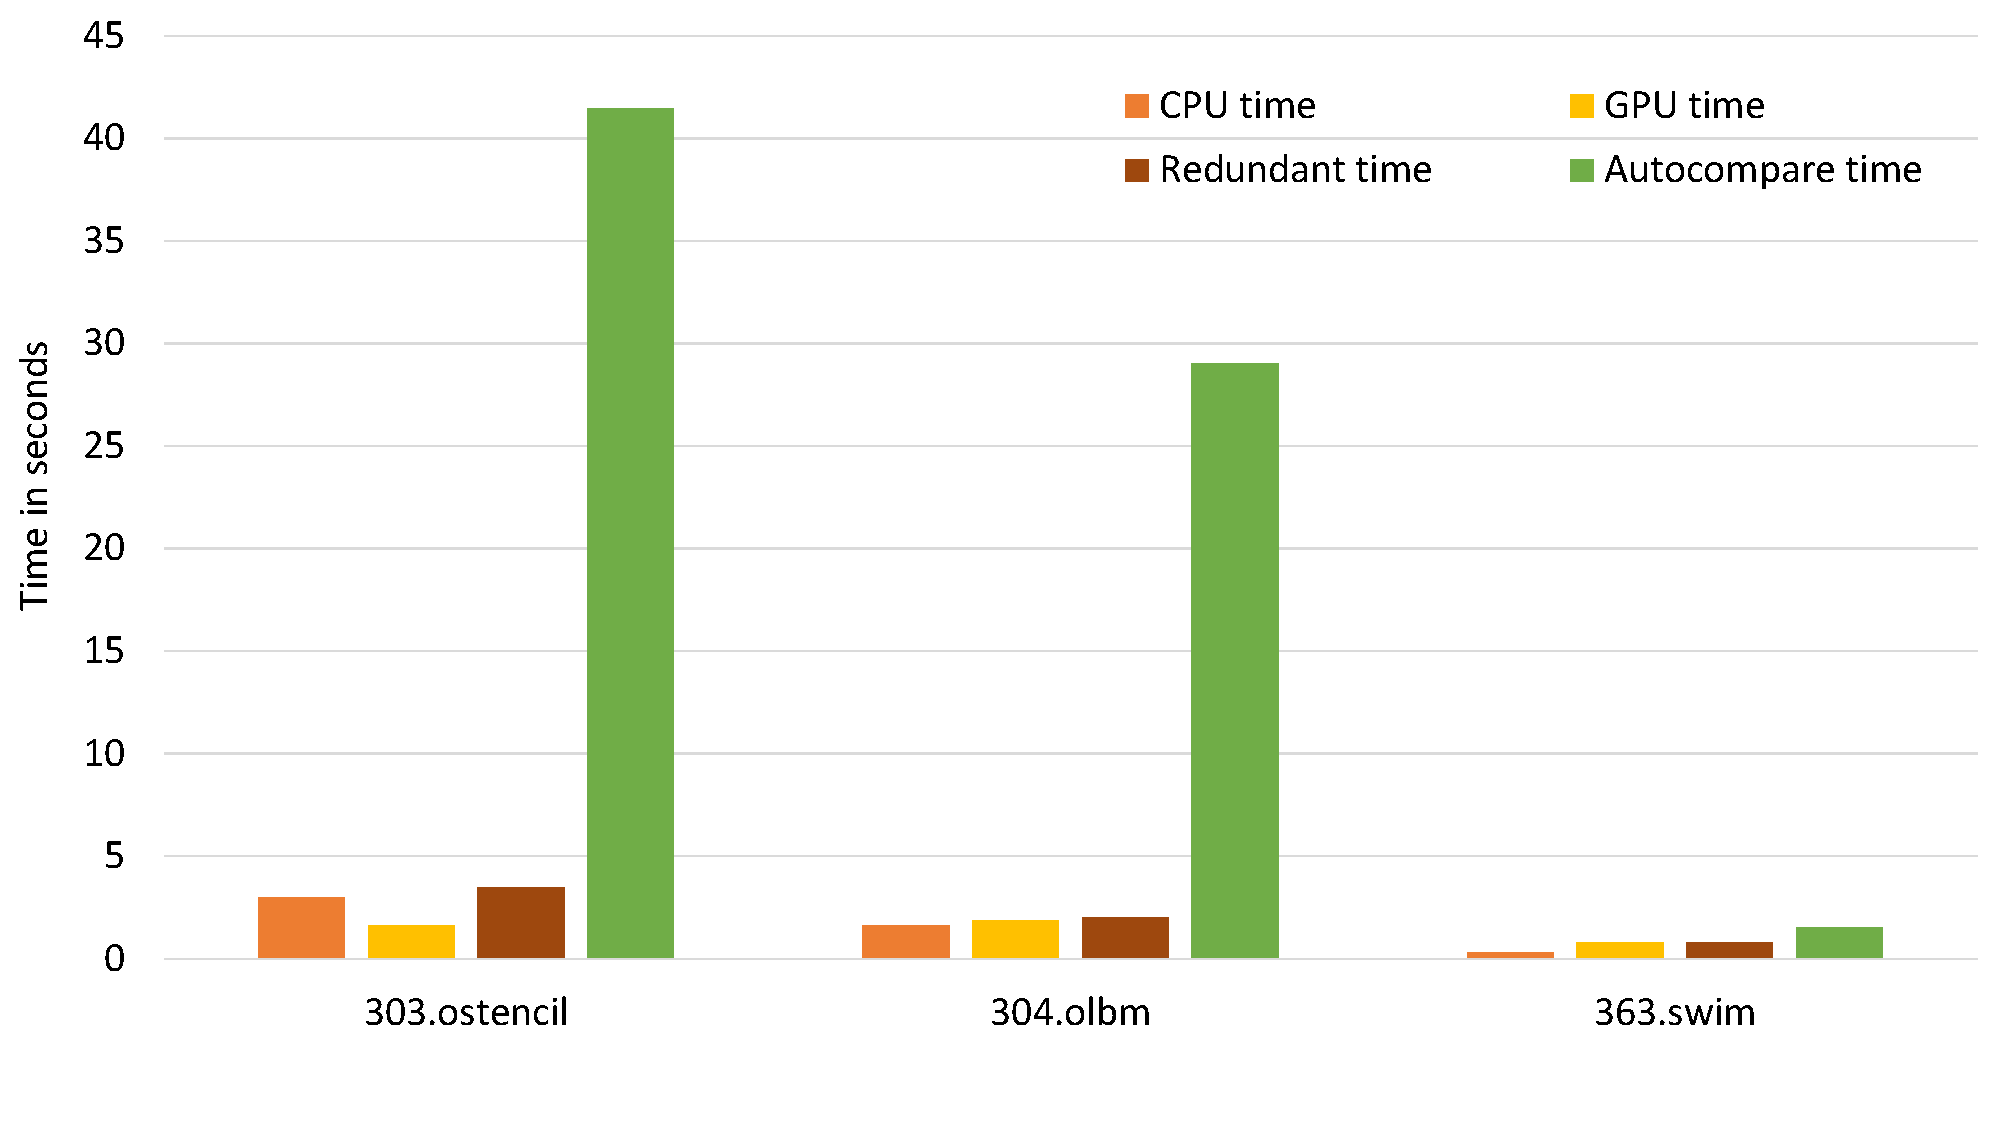
\includegraphics [width=\linewidth] {Table1.pdf}
    \caption{Results showing overhead of OpenACC autocompare.}
    \label{fig:sle_fiure}
\end{figure*}




\begin{table}
\begin{center}
\begin{tabular}{rrrl}
\hline
303.ostencil & 304.olbm & 363.swim & \\
\hline
 3.01 &  1.61 & 0.33 & CPU time \\
 1.61 &  1.85 & 0.78 & GPU time\\
41.46 & 29.05 & 1.53 & autocompare time \\
202 & 61 & 258 & variables and arrays compared \\
3,388,997,632 & 1,586,800,000 & 67,897,602 & items compared \\
\hline
\end{tabular}
\end{center}
\caption{Results showing overhead of OpenACC autocompare.}
\label{res1}
\end{table}

The two costs of the autocompare feature are running the program on both CPU and GPU, and downloading and comparing the values.
Even compared to sequential CPU time, the overhead is significant, and seems directly related to the number of words or elements compared.
However, using this feature to find where a GPU computation diverges moves the cost from the programmer to the computer, so it could be invaluable regardless of the overhead.
One side note: the \emph{test} datasets are relatively small.
Even so, we had to set the relative tolerance to avoid the comparisons detecting differences due to different summation accumulation order.

\section{Related Work}


The PCAST OpenACC autocompare feature is similar in some respects to redundant execution strategies, which are typically used to detect failing hardware or erroneous software.
The Tandem NonStop computers~\cite{bartlett.tandem.86} implemented redundant execution on identical hardware with automatic checking; the system could detect faulty hardware and fail-over to another processor.
The NASA Space Shuttle carried five computers~\cite{fraser.astro.74}; four of these comprised the primary system and ran identical software with a voting protocol to detect a failing computer.
If the four primary system computers could not determine a correct result, the fifth backup system was enabled for ascent and landing.
The major difference is the autocompare feature assumes that the CPU execution is correct, and it compares the GPU computations to those assumed correct results.

The Cray Comparative Debugger (CCDB)~\cite{derose.sc.15} allows a programmer to launch two versions of a program, such as a CPU-only version and a GPU-accelerated version, and to inspect and compare values between the two versions.
The programmer can also add breakpoints and have the debugger compare specific values between the two program versions when each reaches the breakpoint.
This is perhaps the most aggressive approach to allow value comparisons between two running executions and allows a user to inspect the program when the values diverge, although the comparisons themselves are not performed automatically.

Research using the OpenARC compiler framework~\cite{lee.hpdc.14} has explored several strategies for debugging OpenACC programs~\cite{lee.ipdps.14}.
One mechanism is very much like the PCAST autocompare feature, where the compiler generates device code and host sequential code for specific compute regions.
The user selects specific compute regions to verify, and the rest of the program is executed sequentially by the host CPU, including other compute regions.
All the data is copied from the system memory to the GPU before those selected kernels, and all modified data is copied back and compared afterward.
That work allows more fine grain control of which compute regions to compare, but does not allow for a unified framework to run the whole program and compare data after each compute region.

\section{Future Work}

We are considering future work on the autocompare feature, including:
\begin{itemize}
\item Optimizing the comparison operation, since this seems to be the bottleneck for the autocompare feature.
\item Ways to reduce the number of values being compared, to reduce the runtime cost.
\item Running the compare itself in parallel, and perhaps running the compare code on the GPU itself.
\item Some way to isolate regions of the program that are being tested, so as to not require redundant execution and data compares throughout the whole execution.
\item Running the host code in parallel as well, for performance, though this assumes that host parallel execution is as accurate and precise as the host sequential execution.
\item Adding support for arrays of structs or arrays of derived types, where each field would have a type-specific compare.
\item Adding support for nested data structures, where a struct memory is a pointer to another array.
The compare function would recurse to compare the nested structure as well.
\end{itemize}

\section{Conclusion}

While directive based GPU programming models improve the productivity of GPU programming, they do not ensure correctness or the absence of logical errors.
These programming models usually consist of several compiler optimizations and transformations that are hidden from the programmer.
These models improve productivity but unfortunately present challenges to users who must debug and verify program correctness.
This work, part of the PCAST feature, can automatically detect numerical differences that can occur due to computational differences on different OpenACC devices.
Hence, PCAST can automatically check the correctness of an OpenACC implementation and it can also help to identify bugs in OpenACC data management and computation and support programmers in the development of OpenACC applications.

The overhead incurred due to redundant execution is dominated by the slower execution unit and is relatively small, while the overhead of the compare operation is significant.
However, automatic debuggers and correctness checkers always introduce some overhead, and in most cases the total cost is much less than manual investigation.

%


%\section{Obstacles for Unit Tests in HPC}

%\section {What Problems are addressed}
%\subsection{comparing results between a known good version (golden) and a version being tested}
%  - deciding what values to save / compare
%  - deciding when to save / compare values
%  - deciding how to do the compare, esp. for floating point
%\subsection{Usage Scenarios}
%  - user driven, save golden values to a file, compare test version against those
%    using API calls or directives
%    user decides what values to save/compare, when to compare
%  - automatic online compare, compare CPU vs GPU computations
%    can either compare after each kernel launch, or
%    compare all values present on device against golden host values

%\section{Implementation Details}
%   compare options - tolerance, IEEE comparisons
%   where in the runtime it is implemented (?)
%   challenges: Fortran vs C, gcc-specific header file functionality
%   saving a golden file, file block headers to compare execution sequence

%\section{Experimentation}
%   cost overhead of compare
%   cost overhead of autocompare
%   what kinds of differences we find
%
%\section{Other Uses of a Compare Feature}
%   compare different algorithms
%   compare compiler optimizations
%   compare different hosts

\bibliographystyle{IEEEtran}
\bibliography{main}



\end{document}
